% Independent research proposal. pdfLaTeX, two passes. No external figures.
\documentclass[aspectratio=169,10pt]{beamer}
\usepackage[english]{babel}
\usepackage[utf8]{inputenc}
\usepackage[T1]{fontenc}
\usepackage{lmodern,amsmath,booktabs,tabularx,array,tikz}
\usepackage{colortbl}
\usetikzlibrary{arrows.meta}
\usetheme{Madrid}
\definecolor{Ink}{HTML}{243748}
\definecolor{Muted}{HTML}{667B8B}
\definecolor{Accent}{HTML}{347E74}
\definecolor{AccentBlue}{HTML}{507DAD}
\definecolor{SoftMint}{HTML}{E6F4EE}
\definecolor{SoftLilac}{HTML}{F1EEF8}
\definecolor{Paper}{HTML}{FBFCFE}
\setbeamercolor{background canvas}{bg=Paper}
\setbeamercolor{normal text}{fg=Ink}
\setbeamercolor{structure}{fg=Accent}
\setbeamercolor{frametitle}{fg=Ink,bg=Paper}
\setbeamercolor{footline}{fg=Muted,bg=Paper}
\setbeamercolor{mintbox}{fg=Ink,bg=SoftMint}
\setbeamercolor{lilacbox}{fg=Ink,bg=SoftLilac}
\setbeamerfont{frametitle}{size=\large,series=\bfseries}
\setbeamertemplate{headline}{}
\setbeamertemplate{navigation symbols}{}
\setbeamertemplate{frametitle}{\nointerlineskip
\begin{beamercolorbox}[wd=\paperwidth,ht=.74cm,dp=.14cm,leftskip=.55cm]{frametitle}
\usebeamerfont{frametitle}\insertframetitle\end{beamercolorbox}}
\setbeamertemplate{footline}{\begin{beamercolorbox}[wd=\paperwidth,ht=.30cm,dp=.16cm,rightskip=.48cm]{footline}
\hfill\scriptsize Research Direction\enspace |\enspace\insertframenumber\,/\,\inserttotalframenumber\end{beamercolorbox}}
\setbeamersize{text margin left=.48cm,text margin right=.48cm}
\newcommand{\noteurl}{https://app.notion.com/p/412c9399c91881fa90a4c56a96ce42d6}
\newcommand{\notes}[1]{\href{\noteurl}{Research record, #1}}
\newcommand{\card}[3]{\begin{beamercolorbox}[wd=\linewidth,rounded=true,sep=.10cm]{#1}
{\small\bfseries\color{Accent}#2}\par\vspace{.06cm}{\footnotesize\raggedright #3\par}\end{beamercolorbox}}
\newcommand{\lead}[2]{\par\vspace{.08cm}{\bfseries\color{Accent}#1}\quad #2\par}
\hypersetup{pdftitle={Power-Aware HBM/HBF Co-Design for Disaggregated MoE Serving},pdfauthor={Yu-Jui Liang}}
\newcommand{\dimensionrow}[3]{\begin{beamercolorbox}[wd=\linewidth,sep=.08cm,rounded=true]{#1}
\small\makebox[1.65cm][l]{\textbf{\color{Accent}#2}}\parbox[t]{12.65cm}{\raggedright #3}
\end{beamercolorbox}\vspace{.06cm}}

\begin{document}

% Independent, unnumbered cover. The six content frames remain 1/6--6/6.
\begin{frame}[plain,noframenumbering]
\vspace{.55cm}
{\small\bfseries\color{Accent}RESEARCH DIRECTION\par}
\vspace{.38cm}
{\LARGE\bfseries Power-Aware HBM/HBF Co-Design\par}
\vspace{.12cm}
{\LARGE\bfseries for Disaggregated MoE Serving\par}
\vspace{.38cm}
{\color{Accent}\rule{2.2cm}{1.2pt}\par}
\vspace{.30cm}
{\large Yu-Jui Liang\quad Advisor: Hsiang-Yun Cheng\par}
\vspace{.12cm}
{\color{Muted}National Taiwan University / Academia Sinica\par}
\vspace{.35cm}
{\large Research Meeting\quad 11 November 2026\par}
\vfill
{\small\color{Muted}Proposed research direction\par}
\vspace{.35cm}
\end{frame}


\begin{frame}[t]{Proposed Research Direction}
\vspace{.08cm}
\begingroup
\dimensionrow{mintbox}{Hardware}{Heterogeneous GPU HBM/HBF configurations.}
\dimensionrow{lilacbox}{Serving}{Attention/Expert separation, memory residency and scheduling.}
\dimensionrow{mintbox}{Objective}{Improve energy efficiency under latency/SLO and hardware constraints.}
\endgroup
\vspace{.04cm}
{\small\bfseries\color{Accent}Evaluation metrics\par}
\vspace{.05cm}
{\footnotesize
\renewcommand{\arraystretch}{1.0}
\begin{tabularx}{\textwidth}{@{}>{\raggedright\arraybackslash}X >{\raggedright\arraybackslash}p{4cm}@{}}
\toprule
\textbf{Metric} & \textbf{Unit}\\\midrule
Energy per output token & J/token\\
Energy efficiency & tokens/J\\
Time to first token (TTFT) & ms\\
Time per output token (TPOT) & ms/token\\
Goodput under SLO & tokens/s\\
Operational carbon emissions per output token & gCO$_2$e/token\\
\bottomrule
\end{tabularx}\par}
\vspace{.04cm}
{\footnotesize\textbf{Research goal:} Reduce power consumption and carbon emissions across data centers\\
through hardware co-design and coordinated serving, while meeting latency and SLO requirements.\par}
\end{frame}

\begin{frame}[t]{Why Heterogeneous HBM/HBF GPUs?}
\vspace{.10cm}
\small\renewcommand{\arraystretch}{1.35}
\begin{tabularx}{\textwidth}{@{}>{\raggedright\arraybackslash}p{3.0cm} >{\raggedright\arraybackslash}X >{\raggedright\arraybackslash}p{4.05cm}@{}}
\toprule
\textbf{Data} & \textbf{Access behavior} & \textbf{Candidate placement}\\\midrule
\textbf{Active KV cache} & Frequent decode reads, incremental updates. Latency/bandwidth sensitive. & HBM is a natural baseline.\\
\textbf{Hot expert weights} & Read-mostly with frequent reuse. & HBM cache may help.\\
\textbf{Cold expert weights} & Large capacity, read-mostly. & HBF may add residency capacity.\\
\textbf{Intermediate activations} & Transfer between GPU workers. & Explicit network cost and synchronization.\\\bottomrule
\end{tabularx}
\vspace{.25cm}
\card{mintbox}{Research question}{Can role-specific HBM/HBF configurations improve the energy efficiency of MoE serving?}
\vspace{.14cm}
\textbf{Capacity is a possible benefit.}\quad HBF reads and GPU waiting can consume it.\\
HBF does not automatically save power.
\end{frame}

\begin{frame}[t]{Proposed Attention/Expert Architecture}
\relax
{\small\color{Accent}\textbf{Hypothesis to evaluate}\quad Within one data center.\par}
\vspace{.12cm}
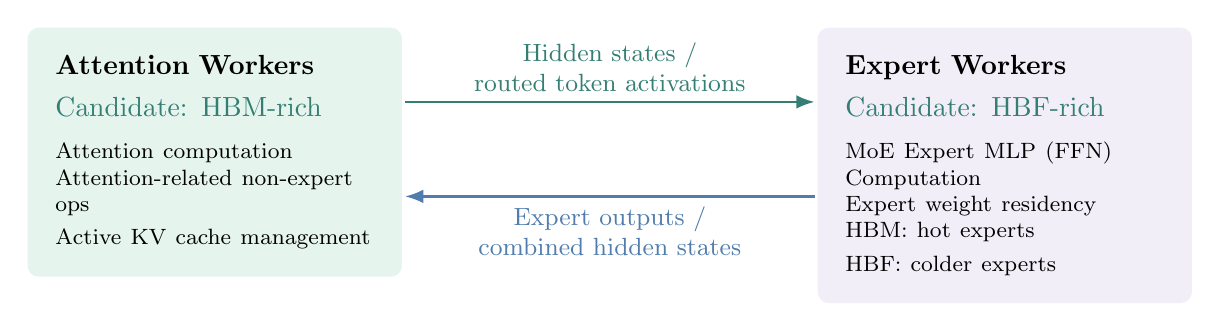
\begin{tikzpicture}[x=1cm,y=1cm,>=Latex]
\node[fill=SoftMint,rounded corners=4pt,inner sep=10pt,text width=4.05cm,minimum height=2.9cm,anchor=north west,align=left] (a) at (0,0) {
\textbf{Attention Workers}\\[3pt]
{\color{Accent}Candidate: HBM-rich}\\[6pt]
\footnotesize Attention computation\\
Attention-related non-expert ops\\
Active KV cache management};
\node[fill=SoftLilac,rounded corners=4pt,inner sep=10pt,text width=4.05cm,minimum height=2.9cm,anchor=north east,align=left] (e) at (14.8,0) {
\textbf{Expert Workers}\\[3pt]
{\color{Accent}Candidate: HBF-rich}\\[6pt]
\footnotesize MoE Expert MLP (FFN)\\Computation\\
Expert weight residency\\
HBM: hot experts\\
HBF: colder experts};
\draw[->,thick,Accent] (4.8,-.95) -- (10,-.95) node[midway,above,align=center,font=\small] {Hidden states /\\routed token activations};
\draw[<-,thick,AccentBlue] (4.8,-2.15) -- (10,-2.15) node[midway,below,align=center,font=\small] {Expert outputs /\\combined hidden states};
\end{tikzpicture}\par
\vspace{.06cm}
{\small\textbf{Residency:} We do NOT transfer the entire historical KV cache or all expert weights\\between worker groups at every layer.\par}
\vspace{.07cm}
\card{mintbox}{Costs remain}{Activation communication, synchronization and HBF read stalls may dominate performance.}
\vspace{.12cm}
\end{frame}

\begin{frame}[t]{Proposed Simulation Integration Stack}
\vspace{0cm}
\centering
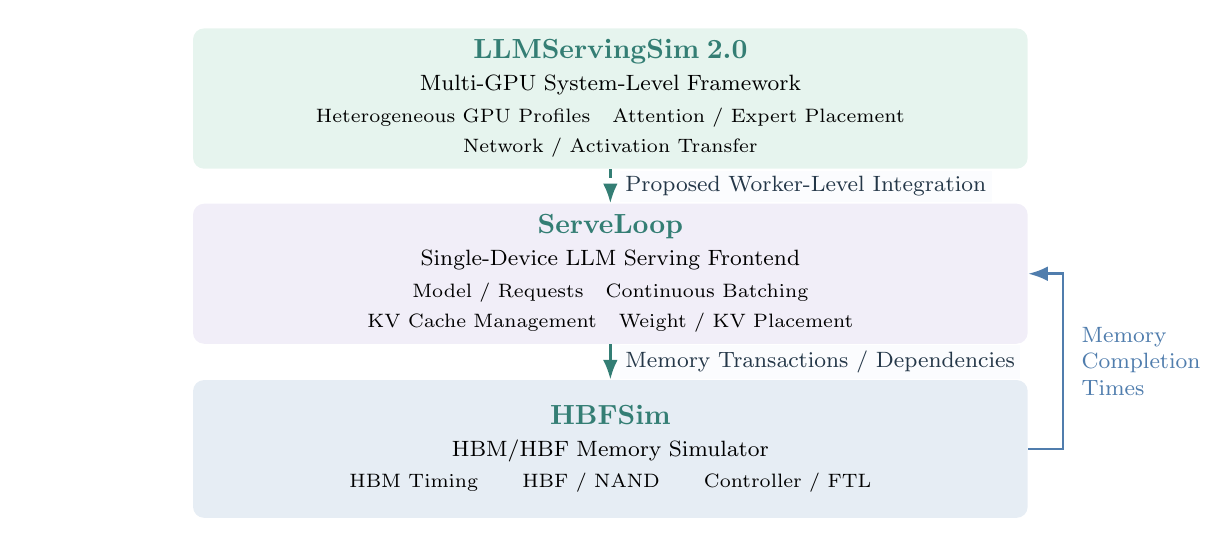
\begin{tikzpicture}[x=1cm,y=1cm,>=Latex,
  stack/.style={rounded corners=4pt,minimum width=10.6cm,minimum height=1.75cm,
    text width=10.1cm,inner sep=4pt,align=center,font=\fontsize{7.5}{10}\selectfont},
  flow/.style={->,line width=.9pt,Accent},
  flowlabel/.style={font=\footnotesize,text=Ink,fill=Paper,inner sep=2pt}]
\path[use as bounding box] (0,.90) rectangle (14.8,-5.35);
\node[stack,fill=SoftMint] (system) at (7.4,0) {
  {\fontsize{10}{11}\selectfont\bfseries\color{Accent}LLMServingSim 2.0}\\[1.5pt]
  {\fontsize{8.5}{10}\selectfont Multi-GPU System-Level Framework}\\[1.5pt]
  Heterogeneous GPU Profiles\quad Attention / Expert Placement\\[1pt]Network / Activation Transfer};
\node[stack,fill=SoftLilac] (serving) at (7.4,-2.225) {
  {\fontsize{10}{11}\selectfont\bfseries\color{Accent}ServeLoop}\\[1.5pt]
  {\fontsize{8.5}{10}\selectfont Single-Device LLM Serving Frontend}\\[1.5pt]
  Model / Requests\quad Continuous Batching\\[1pt]KV Cache Management\quad Weight / KV Placement};
\node[stack,fill=AccentBlue!12!Paper] (memory) at (7.4,-4.45) {
  {\fontsize{10}{11}\selectfont\bfseries\color{Accent}HBFSim}\\[1.5pt]
  {\fontsize{8.5}{10}\selectfont HBM/HBF Memory Simulator}\\[1.5pt]
  HBM Timing\qquad HBF / NAND\qquad Controller / FTL};
\draw[flow,dashed] (system.south) -- (serving.north)
  node[midway,right=3pt,flowlabel] {Proposed Worker-Level Integration};
\draw[flow] (serving.south) -- (memory.north)
  node[midway,right=3pt,flowlabel] {Memory Transactions / Dependencies};
\draw[flow,AccentBlue] (memory.east) -- (13.15,-4.45) -- (13.15,-2.225) -- (serving.east);
\node[font=\footnotesize,text=AccentBlue,align=left,anchor=west,text width=1.45cm]
  at (13.26,-3.3375) {Memory\\Completion\\Times};
\end{tikzpicture}\par
\vspace{.08cm}
{\small\textbf{\color{Accent}Goal:} Evaluate heterogeneous HBM/HBF GPU configurations for Attention--Expert MoE serving.\par}
\vspace{.06cm}
{\footnotesize\itshape\color{Muted}Proposed architecture; multi-GPU integration and energy-model calibration remain future work.\par}
\end{frame}

\begin{frame}[t]{Research Questions and Next Steps}
\vspace{.08cm}
\begin{beamercolorbox}[wd=\linewidth,sep=.15cm,rounded=true]{mintbox}
\small\textbf{\color{Accent}RQ1}\quad
\parbox[t]{13.1cm}{\raggedright Does HBM-rich Attention + HBF-rich Experts beat homogeneous or monolithic alternatives in energy efficiency under the same SLO constraints?}
\end{beamercolorbox}
\vspace{.13cm}
\begin{beamercolorbox}[wd=\linewidth,sep=.15cm,rounded=true]{lilacbox}
\small\textbf{\color{Accent}RQ2}\quad
\parbox[t]{13.1cm}{\raggedright When do HBF read latency, GPU waiting energy and A/E communication outweigh residency benefits?}
\end{beamercolorbox}
\vspace{.13cm}
\begingroup
\setbeamercolor{rqblue}{fg=Ink,bg=AccentBlue!12!Paper}
\begin{beamercolorbox}[wd=\linewidth,sep=.15cm,rounded=true]{rqblue}
\small\textbf{\color{Accent}RQ3}\quad
\parbox[t]{13.1cm}{\raggedright Which configurations give the best energy--goodput trade-off under comparable capacity, package, cost and power constraints?}
\end{beamercolorbox}
\endgroup
\vspace{.16cm}
\card{lilacbox}{NEXT WEEK --- November 18, 2026}{\textbf{MemExplorer: Navigating the Heterogeneous Memory\\Design Space for Agentic Inference NPUs}\\[3pt]
Already explores heterogeneous compute/memory, including HBM/HBF, and energy/performance trade-offs. Study its actual novelty coverage and limitations before finalizing our contribution.\\[3pt]
\textbf{A separate paper-review presentation next week.}}
\end{frame}

\begin{frame}[t]{Related Work Comparison Matrix}
\vspace{.02cm}
{\fontsize{7.5}{9.3}\selectfont
\setlength{\tabcolsep}{3pt}\renewcommand{\arraystretch}{1.30}
\begin{tabularx}{\textwidth}{@{}>{\raggedright\arraybackslash}p{2.65cm}>{\raggedright\arraybackslash}p{3.20cm}>{\raggedright\arraybackslash}p{1.50cm}>{\raggedright\arraybackslash}X >{\raggedright\arraybackslash}p{2.85cm}@{}}
\rowcolor{SoftMint}\textbf{Paper} & \textbf{Simulator / Evaluation} & \textbf{Cross Data Center} & \textbf{Partition / Placement} & \textbf{Objective /\newline (Eval. Metrics)}\\
Helix & Own sim. + GPU cluster & Yes (sim.) & Layers, pipeline, routing & Throughput, latency\\
\rowcolor{SoftLilac}ThunderServe & Estimator + GPU tests & Not shown & P/D, TP/PP; KV & Throughput, perf/\$\\
Hetis & vLLM prototype; sim. NV & Not shown & Attention heads; KV & Throughput, KV use\\
\rowcolor{SoftLilac}Tessera & GPU runtime; sim. NV & Not shown & Kernel placement & Throughput, perf/\$\\
GreenCache & Prototype + replay/model & No & SSD KV/prefix placement & Carbon + SLO\\
\rowcolor{SoftLilac}Janus & Serving runtime; sim. NV & Not shown & A/E pools; experts & Per-GPU throughput\\
How Far Can\newline Disaggregation Go? & Profiles + ASTRA-Sim & Not shown & A/FFN; GPU placement & SLO throughput\\
\rowcolor{SoftLilac}Carbon--SLO & Geo queue/network sim. & Yes & Request / batch routing & Carbon + SLO\\
LLMServingSim 2.0 & Multi-GPU sim. + profiles & Not shown & Heterogeneous TP/PP/EP & (Perf., energy, fidelity)\\
\rowcolor{SoftLilac}HBFSim / ServeLoop & Event-driven / one device & No & Transactions; KV/weights & (Timing, wear/thermal)\\
MemExplorer & Analytical co-design DSE & Not shown & HBM/HBF; P/D, A/FFN & Token/J, performance\\
\rowcolor{SoftLilac}Characterizing HBF & Trace-driven request sim. & Not shown & Multi-GPU; KV/experts & (Time, energy, wear)\\
Potential Applications\newline of HBF & Capacity/replication model & Not shown & Expert residency/replicas & (TPOT, network traffic)\\
\end{tabularx}\par}
\end{frame}
\end{document}
